%!TeX root=../main.tex

\chapter{Tecnologie e strumenti utilizzati}\label{ch:tecnologie-e-strumenti-utilizzati}

La realizzazione del progetto \textbf{Swift Contest} è stata resa possibile dall'adozione di un insieme di tecnologie, piattaforme e strumenti moderni, selezionati per soddisfare i requisiti di cross-platform, sicurezza, scalabilità e velocità di sviluppo.
Questo capitolo descrive lo stack tecnologico utilizzato, giustificando le scelte chiave in relazione agli obiettivi del progetto.

\section{Stack tecnologico principale}\label{sec:stack-tecnologico-principale}
Questa sezione descrive i linguaggi e i framework utilizzati per la scrittura del codice sorgente dell'applicazione, sia lato client che lato server.

\subsection{Frontend: Flutter e Dart}\label{subsec:frontend:-flutter-e-dart}

\begin{wrapfigure}{l}{0.15\textwidth}
    \centering
    \vspace{-\intextsep} % Rimuove spazio extra sopra
    
\includegraphics[width=0.9\linewidth]{capitoli/figure/logos/flutter}
\end{wrapfigure}
\textbf{Flutter} è il framework UI open-source di Google scelto per lo sviluppo dell'applicazione client.
La sua caratteristica principale è la capacità di generare applicazioni compilate nativamente per mobile, web e desktop da un'unica codebase.
Questa scelta è stata fondamentale per soddisfare il requisito di \textbf{sviluppo cross-platform}, garantendo un'esperienza utente coerente e riducendo drasticamente i tempi e i costi di sviluppo e manutenzione.
\vspace{1em} % Aggiunge spazio per separare

\begin{wrapfigure}{l}{0.15\textwidth}
    \centering
    \vspace{-\intextsep}
    
\includegraphics[width=0.9\linewidth]{capitoli/figure/logos/dart}
\end{wrapfigure}
\textbf{Dart} è il linguaggio di programmazione su cui si basa Flutter.
È un linguaggio moderno, orientato agli oggetti e fortemente tipizzato, ottimizzato per la creazione di interfacce utente.
La sua architettura, che supporta sia la compilazione \emph{Just-In-Time (JIT)} per uno sviluppo rapido (con \emph{hot reload}) sia la compilazione \emph{Ahead-Of-Time (AOT)} per performance elevate in produzione, lo ha reso la scelta naturale per questo progetto.

\subsection{Backend: Supabase, PL/pgSQL e TypeScript}\label{subsec:backend:-supabase-pl/pgsql-e-typescript}

\begin{wrapfigure}{l}{0.15\textwidth}
    \centering
    \vspace{-\intextsep}
    
\includegraphics[width=0.9\linewidth]{capitoli/figure/logos/supabase}
\end{wrapfigure}
\textbf{Supabase} è la piattaforma open-source \textbf{Backend-as-a-Service (BaaS)} che costituisce il cuore dell'infrastruttura server.
La scelta è ricaduta su Supabase dopo un'attenta valutazione delle principali alternative, in particolare \textbf{Firebase} di Google.
Sebbene entrambe le piattaforme offrano un set di funzionalità simile (autenticazione, storage, funzioni serverless), Supabase è stato preferito per una ragione architetturale fondamentale: il suo database è \textbf{PostgreSQL}, un sistema \emph{SQL} maturo e relazionale.
Questa caratteristica è stata ritenuta cruciale per un'applicazione con un modello dati complesso e interconnesso come Swift Contest, dove la garanzia di integrità referenziale e la possibilità di eseguire query complesse sono requisiti fondamentali.
Supabase offre, in un'unica soluzione integrata, tutti i servizi necessari: un database PostgreSQL completo, un sistema di autenticazione, uno storage per i file, API auto-generate e servizi serverless (RPC ed Edge Functions).
\vspace{1em}

\begin{wrapfigure}{l}{0.15\textwidth}
    \centering
    \vspace{-\intextsep}
    
\includegraphics[width=0.9\linewidth]{capitoli/figure/logos/postgresql}
\end{wrapfigure}
\textbf{PL/pgSQL} è il linguaggio procedurale di PostgreSQL. È stato utilizzato per scrivere tutte le \textbf{Funzioni RPC (Remote Procedure Call)} del sistema.
La scelta di implementare la logica di accesso ai dati direttamente a livello di database tramite questo linguaggio ha permesso di ottenere performance elevate e di garantire l'atomicità delle operazioni, sfruttando al contempo il potente sistema di sicurezza di PostgreSQL\@.
\vspace{1em}

\begin{wrapfigure}{l}{0.15\textwidth}
    \centering
    \vspace{-\intextsep}
    
\includegraphics[width=0.9\linewidth]{capitoli/figure/logos/typescript}
\end{wrapfigure}
\textbf{TypeScript} è stato scelto come linguaggio per lo sviluppo delle \textbf{Edge Functions}, eseguite sul \emph{runtime Deno} di Supabase.
La sua natura fortemente tipizzata, unita alla vasta disponibilità di librerie dell'ecosistema JavaScript/TypeScript, lo ha reso ideale per gestire logiche complesse, transazioni multi-step e, soprattutto, per orchestrare le interazioni sicure con le API di servizi esterni.

\section{Piattaforme, Strumenti e Servizi}\label{sec:piattaforme-strumenti-e-servizi}
Questa sezione descrive le piattaforme di terze parti e gli strumenti che hanno supportato il ciclo di vita del progetto.

\subsection{Piattaforme di Deployment e Servizi Cloud}\label{subsec:piattaforme-di-deployment-e-servizi-cloud}

\begin{wrapfigure}{l}{0.15\textwidth}
    \centering
    \vspace{-\intextsep}
    
\includegraphics[width=0.9\linewidth]{capitoli/figure/logos/vercel}
\end{wrapfigure}
\textbf{Vercel} è la piattaforma serverless utilizzata per il deployment e l'hosting della versione \textbf{Web} dell'applicazione Flutter.
La scelta è ricaduta su Vercel principalmente per il suo \textbf{piano gratuito}, che ha permesso di distribuire l'applicazione senza sostenere costi.
Oltre a questo, Vercel è stato preferito per le sue caratteristiche tecniche di alto livello, come l'integrazione nativa con i framework frontend moderni e una pipeline di \textbf{CI/CD} completamente automatizzata.
\vspace{1em}

\begin{wrapfigure}{l}{0.15\textwidth}
    \centering
    \vspace{-\intextsep}
    
\includegraphics[width=0.9\linewidth]{capitoli/figure/logos/resend}
\end{wrapfigure}
\textbf{Resend} è il servizio transazionale di invio \textbf{email} utilizzato dal sistema.
È stato integrato tramite la propria API REST, invocata da una Edge Function, per gestire l'invio di tutte le email automatiche, come gli inviti per partecipanti e giurati.
\vspace{1em}

\begin{wrapfigure}{l}{0.15\textwidth}
    \centering
    \vspace{-\intextsep}
    
\includegraphics[width=0.9\linewidth]{capitoli/figure/logos/google-cloud}
\end{wrapfigure}
\textbf{Google Cloud} è stato utilizzato per uno dei suoi servizi API: la \textbf{Google Places API}.
Questo servizio è stato integrato per fornire la funzionalità di ricerca e autocompletamento degli indirizzi nella creazione dei contest e nella configurazione delle sessioni di voto per la geolocalizzazione.

\subsection{Strumenti di Sviluppo e Amministrazione}\label{subsec:strumenti-di-sviluppo-e-amministrazione}

\begin{wrapfigure}{l}{0.15\textwidth}
    \centering
    \vspace{-\intextsep}
    
\includegraphics[width=0.9\linewidth]{capitoli/figure/logos/intellij}
\end{wrapfigure}
\textbf{IntelliJ IDEA} è l'IDE di JetBrains utilizzato per la scrittura del codice.
Sebbene lo sviluppo iniziale fosse stato avviato su \textbf{Android Studio}, si è scelto di migrare a \textbf{IntelliJ IDEA Community Edition} per una maggiore stabilità e reattività.
Grazie ai plugin ufficiali, ha offerto un ambiente di sviluppo performante e affidabile per tutti i linguaggi del progetto.
\vspace{1em}

\textbf{Material Theme Builder} è uno strumento ufficiale di Google, disponibile online e su Figma, che è stato utilizzato per generare la base del tema Material Design 3.
A partire da un singolo colore ``seme'' (seed color), lo strumento genera automaticamente l'intera palette di colori (\texttt{ColorScheme}) per il tema chiaro e scuro, garantendo coerenza cromatica e accessibilità.
Il codice Dart generato da questo strumento è stato poi utilizzato come base per il \texttt{MaterialTheme} dell'applicazione, arricchito successivamente con estensioni personalizzate.
\vspace{1em}

\begin{wrapfigure}{l}{0.15\textwidth}
    \centering
    \vspace{-\intextsep}
    
\includegraphics[width=0.9\linewidth]{capitoli/figure/logos/npm}
\end{wrapfigure}
\textbf{Node Package Manager (npm)} è stato uno strumento indispensabile per l'installazione e la gestione di dipendenze di sviluppo, prima tra tutte la \textbf{CLI di Supabase}, utilizzata per gestire le migrazioni del database e il deployment delle Edge Functions.
\vspace{1em}

\begin{wrapfigure}{l}{0.15\textwidth}
    \centering
    \vspace{-\intextsep}
    
\includegraphics[width=0.9\linewidth]{capitoli/figure/logos/retool}
\end{wrapfigure}
\textbf{Retool} è la piattaforma \emph{low-code} utilizzata per costruire rapidamente la \textbf{dashboard di amministrazione} interna.
La sua capacità di interfacciarsi in modo nativo e sicuro con database PostgreSQL e API REST ha permesso di creare uno strumento di moderazione funzionale in poche ore.

\subsection{Version Control e Code Hosting}\label{subsec:version-control-e-code-hosting}

\begin{wrapfigure}{l}{0.15\textwidth}
    \centering
    \vspace{-\intextsep}
    
\includegraphics[width=0.9\linewidth]{capitoli/figure/logos/git}
\end{wrapfigure}
\textbf{Git} è il sistema di \textbf{controllo di versione distribuito} utilizzato per tracciare ogni modifica al codice sorgente del progetto.
La sua adozione è stata fondamentale per gestire lo sviluppo in modo strutturato, permettendo la creazione di branch per nuove funzionalità e la gestione dei merge.
\vspace{1em}

\begin{wrapfigure}{l}{0.15\textwidth}
    \centering
    \vspace{-\intextsep}
    
\includegraphics[width=0.9\linewidth]{capitoli/figure/logos/github}
\end{wrapfigure}
\textbf{GitHub} è la piattaforma di \textbf{code hosting} che ospita il repository Git del progetto.
Oltre al semplice hosting, è stata utilizzata per la sua integrazione con la pipeline di CI/CD di Vercel e per ospitare in modo sicuro le release dell'applicazione Android (APK).

\subsection{Strumenti di Documentazione e Modellazione}\label{subsec:strumenti-di-documentazione-e-modellazione}

\begin{wrapfigure}{l}{0.15\textwidth}
    \centering
    \vspace{-\intextsep}
    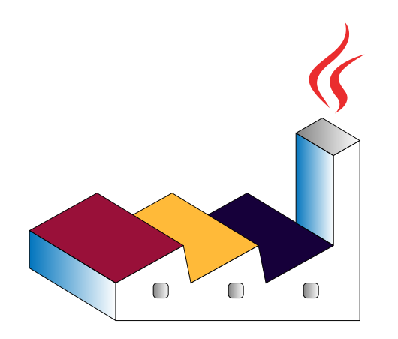
\includegraphics[width=0.9\linewidth]{capitoli/figure/logos/plantuml}
\end{wrapfigure}
\textbf{PlantUML} è lo strumento open-source utilizzato per creare tutti i diagrammi UML e architetturali.
La sua caratteristica distintiva è l'approccio ``diagrams as code'': i diagrammi vengono descritti attraverso un \textbf{linguaggio DSL (Domain-Specific Language)} testuale, permettendo di creare diagrammi versionabili, facilmente modificabili e stilisticamente coerenti.
